\documentclass[11pt]{scrartcl}
\usepackage[sexy]{{style_files/evan}}

\usepackage{{style_files/NMC}}
\usepackage[subpreambles=true]{standalone}
\usepackage{import}

\begin{document}
\title{NMC Problem Set \#2}
\date{Aug. 28, 2022} 
\maketitle

\section*{Welcome!}

This is a selection of classic beginner level Olympiad problems, curated so you can nibble on them throughout the week! The point of this document is to introduce you to fun puzzles that require thinking. We recommend you try problems that you find interesting! Feel free to work on them with others (even us teachers!). Harder problems are marked with chilies (\fullchili), in case you want to challenge yourself.
    
Have fun!
    
Note: New variants on these problems may be released throughout the week. Remember to check back once in a while!
    
\section{Algebra}

\textit{
    \begin{flushright}This is the field you're probably the most familiar with. It talks about\\
    \textbf{equations}, \textbf{inequalities}, \textbf{real} (and sometimes complex!) \textbf{numbers}, \textbf{polynomials}...\\
    despite your experience, these problems will require you to think\\
    in new ways not taught in class.\\
    Think creatively!\end{flushright}
}

\begin{enumerate}[label=\textbf{A\arabic*}.]
    \item \textbf{Cake for mathematicians!}\\
    A HUGE cake has been prepared for a competition with $n = 10000$ participants! Participant $1$ received $1/n$ of the cake, participant $2$ received $2/n$ of the \textit{remaining} cake, participant $3$ received $3/n$ of the \textit{remaining} cake, and the pattern continues, until the final participant, who receives whatever is left over.
    
    In the end, who had the largest share of cake?
\end{enumerate}

\newpage
\section{Combinatorics}

\textit{
    \begin{flushright}
    Combinatorics is a branch of mathematics that primarily deals with\\
    \textbf{counting} things in efficient ways, but here we also include \textbf{games}\\
    and other creative problems that don't fit in the other categories.\\
    \end{flushright}
}

\begin{enumerate}[label=\textbf{C\arabic*}.]
    \item \textbf{Pockies for mathematicians!} \newline
    Arky and Lance are playing a game, taking turns eating Pockies. \footnote{let's be real, who knows if "pocky" is count or noncount.}
    \begin{enumerate}
        \item They start with a box of $30$ Pockies. Lance and Arky can take $1$, $2$ or $3$ from the box per turn. Given that the person who takes the last Pocky wins and that Lance has the first move, who has a winning strategy?
        
        \item After the initial Pockies are finished, they order a second box containing $n$ sticks. This time, Lance and Arky agree to only take $1$ or $2$ Pockies at a time. In terms of $n$, how many different ways are there to finish this box? (For example, if $n = 3$, then Arky and Lance can take turns eating either $1+1+1$, $1+2$ or $2+1$ pockies. In this case, there are $3$ ways.)
        
        \item Now, Lance and Arky have a smaller box of just $10$ pockies, but that doesn't stop MPK and Frog from hopping in as well! To stop everyone from being greedy, a player can only take $1$ or $2$ Pockies at a time. The person who takes the last one \emph{loses}. MPK is given the first move, but he just before he starts, he realizes that the others have formed a team to defeat him! Can MPK still win?
        
        \item (\fullchili) After what transpired earlier, Lance and Arky leave to play the Pocky game by themselves. They buy $k$ boxes with $n_1, n_2, \ldots, n_k$ Pockies each. Each turn, someone picks a box and chooses how many sticks they want to take, with no limit on the amount. This time, Arky begins and the person who takes the last Pocky wins. Who has the winning strategy and when?
    \end{enumerate}
\end{enumerate}

\newpage
\section{Geometry}

\textit{
    \begin{flushright}
    Geometry, studied since ancient Greece, is the oldest discipline of mathematics. It concerns \textbf{space}, \textbf{distances}, \textbf{areas}, \textbf{volumes}.\\ Learn the pretty intricacies of the figures below!
    \end{flushright}
}

\begin{enumerate}[label=\textbf{G\arabic*}.]
    \item \textbf{Efficient Construction} \newline
    In this game, you will be given several geometric pictures drawn in black. Your goal is to find a way to draw the red figure using only a straight-edge and a compass. The figures must be drawn with perfect precision, without taking measurements! (You are not allowed to use the notches on your ruler, nor are you allowed to use a protractor.) Consider using auxiliary lines and circles to reach the goal. As an additional challenge, try to minimize the number of steps!

    \begin{enumerate}
        \item \begin{tabular}{L{7cm}  C{5cm}}
            Given the black angle, find a way to draw the red angle bisector, which is the line that divides the black figure in half. & 
            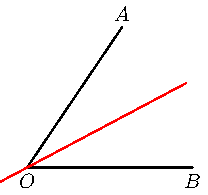
\includegraphics[width = 5cm, page = 1]{Diagrams/W2G1.pdf}
        \end{tabular}
        \item \begin{tabular}{L{7cm}  C{5cm}}
            Given a rectangle and a point $P$ outside of it, find the line that passes through $P$ and divides the rectangle into two equal area halves. & 
            \includegraphics[width = 5cm, page = 2]{Diagrams/W2G1.pdf}
        \end{tabular}
        \item \begin{tabular}{L{7cm}  C{5cm}}
            Given a circle, find its center. & 
            \includegraphics[width = 5cm, page = 3]{Diagrams/W2G1.pdf}
        \end{tabular}
    \end{enumerate}
\end{enumerate}

\newpage
\section{Number Theory}

\textit{
    \begin{flushright}
    Number theory is the part of mathematics that deals with the\\ \textbf{integers} (numbers w/ no decimal dot), \textbf{factorization}, \textbf{divisibility}, \textbf{primes}, ...\\ While its objects are simple, don't be deceived,\\ solutions still require a good bit of cleverness!
    \end{flushright}
}

\begin{enumerate}[label=\textbf{N\arabic*}.]
    \item The Fibonacci sequence is a famous sequence of numbers. Here are the first few terms:
    \[ 0, 1, 1, 2, 3, 5, 8, 13, ... \]
    Let's define a function $F$ that tells us the $n$th Fibonacci number. It starts with $F(0) = 0$ and $F(1) = 1$, and any subsequent number is the sum of the two that precedes it. So for example $F(3) = F(2) + F(1) = 1 + 1 = 2$. It is known that the sequence satisfies many interesting properties, of which some are outlined below!
    \begin{enumerate}
        \item Prove that any two consecutive numbers in the Fibonacci sequence are coprime: they have no factors in common, aside from $1$.
        \item Exactly which numbers of this sequence are even? Which numbers are a multiple of $5$? Which numbers are a multiple of $7$?
        \item Show that $F(2n)$ is a multiple of $F(n)$ for all positive integers $n$.
        \item Show that if you add up the first Fibonacci numbers up to $F(n)$, the result is one less than $F(n+2)$:
        \[ F(0) + F(1) + F(2) + ... + F(n) = F(n+2)-1. \]
    \end{enumerate}
\end{enumerate}

\end{document}
